\documentclass[pdftex,12pt,letter]{article}
\usepackage{fancyhdr}
\usepackage{enumerate}
\usepackage{tabularx}
\usepackage{graphicx}
\usepackage{caption}
\usepackage{subcaption}
\usepackage{array}
\usepackage[toc,page]{appendix}
\usepackage[justification=justified,singlelinecheck=false]{caption}
\usepackage{placeins}
\usepackage{hyperref}
\pagestyle{fancy}
\makeatletter
  \renewcommand\@seccntformat[1]{\csname the#1\endcsname.\quad}
\makeatother

\newcolumntype {Y}{ >{\raggedright \arraybackslash }X}
\newcommand{\HRule}{\rule{\linewidth}{0.5mm}}
\captionsetup{labelformat=empty}

\begin{document}

\begin{titlepage}
\begin{flushright}
\HRule \\[0.4cm]
{ \bfseries
{\huge EECS 405 Final Report\\[1cm]}
{\Large for\\[1cm]}
{\large Improving Efficiency of String Similarity Searches through Clustered Pruning\\[3cm]}
{\large Prepared by\\[1cm]James Fitzpatrick\\Kyle Patterson\\[2cm]
Version 1.0\\
May 2, 2014\\
}}
\end{flushright}
\end{titlepage}

\tableofcontents
\newpage

\section{Abstract}
Inconsistencies in data sets can often interfere . We propose merging the realms of data mining and similarity queries to reduce search times in large data sets while maintaining high accuracy in similarity query results.

\section{Introduction}
String similarity search is a rapidly growing area of research within the computer science community due to its numerous overlapping applications in the modern world. From biology and genetics to computer security, improvements to current string searching techniques must be improved to handle the large amounts of data being gathered today.  As presented in [2], pruning techniques were effective in reducing the time of a query to less than 50 milliseconds; however, these pruning techniques were computationally costly, requiring a minimum of 0.1 billion entries in generated triples in the range-based pruning methods. With the move towards big data sets, it may be more beneficial to include common data-mining practices that are already designed for large sets of data.

\section{Problem Definition}


We propose a method of pruning the search space that utilizes a common data mining technique, clustering. Using the BIRCH clustering algorithm, we will create a heirarchical cluster within the data space based off of edit distance. These clusters will be indexed according to Longest Common Subsequence; when a string query is performed, we will search this cluster heirarchy to find an appropriate subspace of data. The query algorithms, namely the B\textsuperscript{ed}-Tree, Top-\textit{k}, and VGRAM techniques from [1] [2] and [3], will then be restricted to this data subspace; this effectively prunes the search space according to edit distance, without requiring that the algorithms compute the edit distances at each query. \\
\\
We will compare the execution times of our proposed pruning technique versus a na\"{i}ve implementation of the B\textsuperscript{ed}-Tree, Top-\textit{k}, and VGRAM algorithms from [1] [2] and [3]. We hypothesize that by pruning off large clusters of data, a large reduction in query time will be seen.

\section{Related Work}


\section{Methodology}
\subsection{Data preparation}
Data was mirroed from the Database and Logic Programming bibliography (DBLP) and International Movie Database (IMDB) public sources to a MySQL server hosted on a micro instance of Amazon Elastic Cloud Computing (EC2). Data was cleaned to remove any incomplete entries, and trimmed to remove any entries that contained any non-standard ASCII characters (i.e, characters whose value is greater than 127).\\
\\
In total, the IMDB database contained 55,743 movie entries while the DBLP database contained 2,502,896 publication entries.


\subsection{Development Machines}
Tries and tests were constructed and executed on a 64-bit Dell Latitude computer with 8 GB of RAM and an i7-2720QM quad-core processor operating at 2.20 GHz. Algorithms were developed using C\# and executed in the Visual Studio 2013 v12 Runtime Environment. 

\subsection{Cluster identification}
Originally, we had planned to identify clusters among large data sets by using the BIRCH clustering algorithm to develop a heirarchical structure of clusters, similar to the B\textsuperscript{+}-tree structure. However, we had not anticipated 
\\
\\
Strings were indexed according to longest common substring, using a multi-layered inverted list. Due to the large 

\subsection{Testing}
Tests were evaluated using the following method:

\begin{enumerate}
\item Generate query structure for a randomized subset of data
\item Select random values from data subset and randomly edit values within $k$ edits
\item Query trie structure for edited values
\end{enumerate}

Tests were executed for data subsets in increments of 10,000 from 10,000 elements to the full data set, with 30 queries executed per trie. Query structures used include VGRAM and Top-K Tries.

\section{Evaluation}


\section{Results}
\subsection{Cluster generation}
Clustering

\begin{figure}[h!]
\centering
\begin{subfigure}[b]{0.45\textwidth}
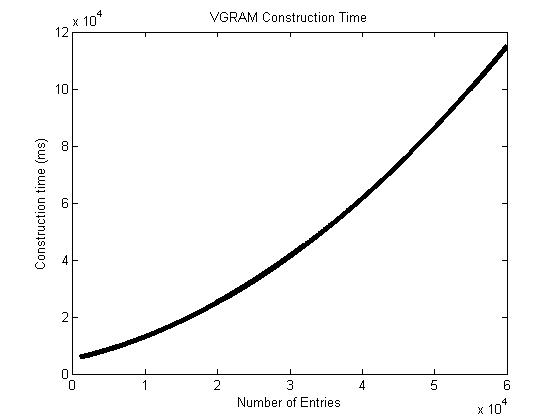
\includegraphics[width=\textwidth]{VGRAMconstructionTime.jpg}
\label{fig:vgram}
\end{subfigure}
\begin{subfigure}[b]{0.45\textwidth}
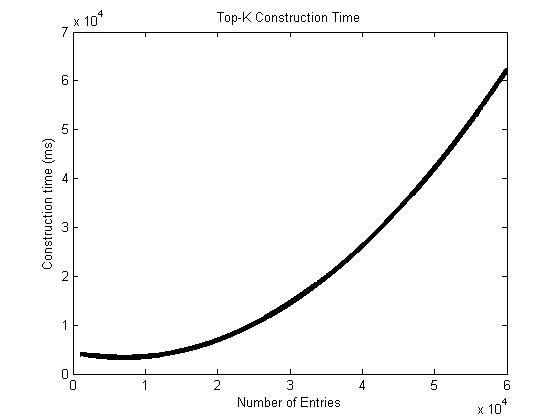
\includegraphics[width=\textwidth]{TOPKconstructionTime.jpg}
\label{fig:topk}
\end{subfigure}
\begin{center}
Figure 1: Construction times for VGRAM and Top-K per data set sizes.
\end{center}
\end{figure}

\begin{figure}[h!]
\centering
\begin{subfigure}[b]{0.45\textwidth}
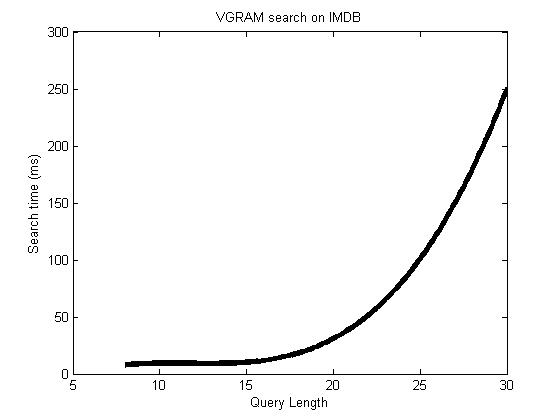
\includegraphics[width=\textwidth]{VGRAMonIMDB.jpg}
\label{fig:imdb}
\end{subfigure}
\begin{subfigure}[b]{0.45\textwidth}
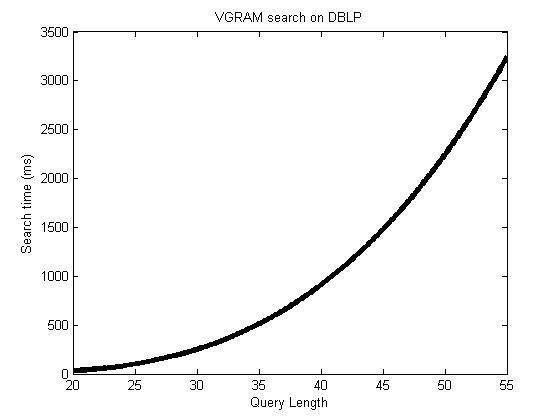
\includegraphics[width=\textwidth]{VGRAMonDBLP.jpg}
\label{fig:dblp}
\end{subfigure}
\begin{center}
Figure 2: Query times per IMDB and DBLP data sets using the VGRAM Trie.
\end{center}
\end{figure}

\begin{figure}[h!]
\centering
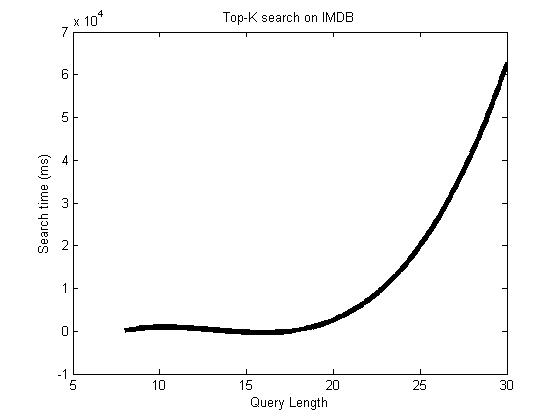
\includegraphics[width=0.5\textwidth]{TOPKonIMDB.jpg}
\begin{center}
Figure 3: Query times for IMDB data set using the Top-K Trie. The full DBLP data set was too large for Top-K queries.
\end{center}
\end{figure}


\section{Conclusions}
In this paper, we presented a pruning technique that relies on common data mining and indexing techniques




\FloatBarrier
\end{document}